\section{Resultate und Diskussion}

Die berechneten Werte sind  als  Tabelle  und  grafisch  zusammengefasst  (siehe
Tabelle \ref{tab:zusammenfassung} und  Abbildung \ref{fig:einzelmessungen}).

\begin{table}[ht!]
    \begin{center}
        \caption{Zusammenfassung der errechneten Werte}
        \label{tab:zusammenfassung}
        \begin{tabular}{lrrr}
            \toprule
            Messmethode & Plank'sche Konstanten \\
            \midrule
            Photospannungsmethode & $\left(5.49771 \pm 1.65266\right)e-34$ \\
            Gegenfeldmethode      & $\left(5.24227 \pm 1.58724\right)e-34$ \\
            Knickspannung         & $\left(7.54210 \pm 2.55475\right)e-34$ \\
            \midrule
            Gewichteter Mittel    & $\left(5.72891 \pm 1.04469\right)e-34$ \\
            \bottomrule
        \end{tabular}
    \end{center}
\end{table}

\begin{figure}[ht!]
    \centering
    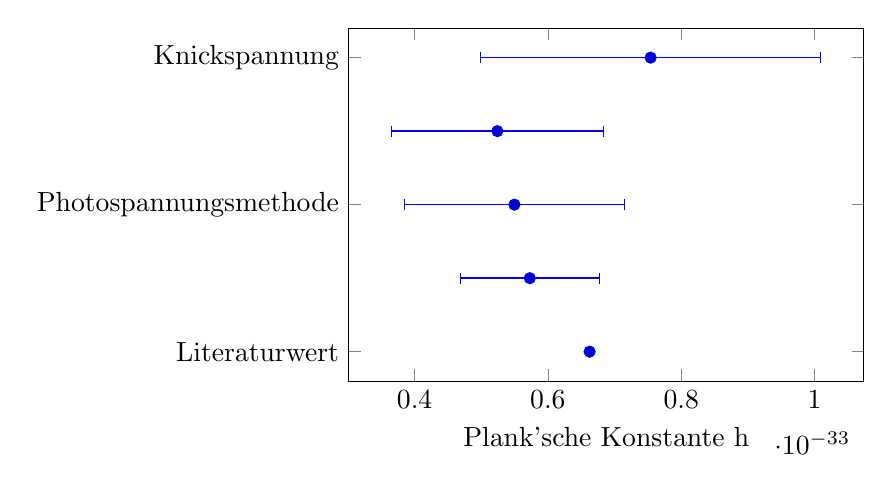
\begin{tikzpicture}
        \begin{axis}[
            width=.67\textwidth,
            height=.5\textwidth,
            xlabel = {Plank'sche Konstante h},
            symbolic y coords = {Literaturwert,
                                 Gewichteter Mittel,
                                 Photospannungsmethode,
                                 Gegenfeldmethode,
                                 Knickspannung},
        ]
        \addplot+[
            only marks,error bars/.cd,
            x dir=both,x explicit,
            error bar style={line width=0.5pt},
            ]
        coordinates {
            (5.49771e-34,Photospannungsmethode) +- (1.65266e-34,0)
            (5.24227e-34,Gegenfeldmethode)      +- (1.58724e-34,0)
            (7.54210e-34,Knickspannung)         +- (2.55475e-34,0)
            (5.72891e-34,Gewichteter Mittel)    +- (1.04469e-34,0)
            (6.626068e-34,Literaturwert)
        };
        \end{axis}
    \end{tikzpicture}
    \caption{Grafische Darstellung der Messungen}
    \label{fig:einzelmessungen}
\end{figure}

Bei   der    Gegenfeldmethode    liegen   die   Messwerte   eher   unter   dem
Literaturwert\cite{ref:h}. Bei den LED-Messungen lag der Messwert start \"uber
dem  Literaturwert. Wie schon erw\"ahnt  unterliegen  diese  Messungen  vielen
systematischen Fehler.

Bei der Messung der Photospannung war die Spannung  extrem  abh\"angig  davon,
wie die Spektrallinien auf den Sensor  ausgerichtet  wurden und wie schmal die
Spaltbreite eingestellt wurde. Weiter  musste  man recht lange warten, bis die
Spannung stabil wurde und auch dann schwankte sie stark.

Die Messung der Knickspannung bei den  LEDs  war  sehr  grob,  haupts\"achlich
wegen der ungenauen Aufl\"osung des Oszilloskops  aber  auch  wegen  der nicht
allzu  starken Ansteigung der  U-I-Kennlinie.  Eine  genauere  Definition  der
Knickspannung und eine genauere analyse der Kennlinie  (z.B. durch abspeichern
der  Messpunkte  und  Evaluation in MATLAB) kann  sicher  ein  viel  genauerer
Messwert gewonnen werden.

